\section{Einführung und Ziele}\label{sec: einfuehrung-und-ziele}
In diesem Abschnitt erfolgt eine Einführung in das Lagersystem, seine Architektur und erläutert die Ziele, die das Lagersystem verfolgt.

\subsection{Einführung}\label{subsec: einfuehrung}
Ziel des Lagersystems ist es, die Verwaltung von Zutatenpaketen in einem Lager zu ermöglichen. Dies umfasst die
Platzierung, Entnahme, Verwaltung und Speicherung von Zutatenpaketen sowie die Bearbeitung des Lagers selbst.

\subsection{Ziele}\label{subsec: ziele}
Die Hauptziele des Lagersystems sind:
\begin{itemize}
    \item \textbf{Effiziente Lagerverwaltung:} Das System soll eine effiziente Verwaltung der Lagerbestände ermöglichen, einschließlich der Platzierung und Entnahme von Zutatenpaketen.
    \item \textbf{Flexibilität}: Das System soll durch die Editier-Funktion des Zutatenlagers auf individuelle Lager-Bedürfnisse des Benutzers eingehen können.
    \item \textbf{Sicherheit:} Das System soll bei der Lagerung dafür sorgen, dass keine Zutatenpakete in einem gemeinsamen Ablagebereich gelagert werden, dessen Inhalte sich nicht vertragen. Außerdem soll die Größe überprüft werden, damit es kein Paket gibt, dessen Proportionen die des Ablagebereiches übertreffen und beim Stapeln auf einem weiteren Paket darf das untere Paket nicht schmaler sein.
    \item \textbf{Benutzerfreundlichkeit:} Das System soll eine intuitive Benutzeroberfläche bieten, die eine einfache und schnelle Bedienung ermöglicht.
    \item \textbf{Erweiterbarkeit:} Die Architektur soll flexibel und erweiterbar sein, um zukünftige Anpassungen und Erweiterungen zu unterstützen.
    \item \textbf{Datenintegrität:} Sicherstellung der Datenintegrität bei allen Operationen, insbesondere bei der Speicherung und Verwaltung von Lagerdaten.
    \item \textbf{Zuverlässigkeit:} Das System soll zuverlässig und robust sein, um einen kontinuierlichen Betrieb zu gewährleisten.
\end{itemize}

\section{Randbedingungen}\label{sec: randbedingungen}
Der folgende Abschnitt stellt die Randbedingungen dar, welche bei der Entwicklung des Lagersystems berücksichtigt wurden:

\subsection{Technische Randbedingungen}\label{subsec: technische-randbedingungen}
\begin{itemize}
    \item \textbf{Technologie:} Das System wird in Java implementiert und nutzt bestehende Java-Bibliotheken für die Verwaltung der Lagerdaten.
    \item \textbf{Plattform:} Das System soll auf dem Betriebssystem Linux laufen.
    \item \textbf{Leistung:} Das System muss in der Lage sein, ein großes Zutatenlager effizient zu verwalten, ohne dass die Performance beeinträchtigt wird.
    \item \textbf{Sicherheit:} Die Daten müssen gegen unbefugten Zugriff geschützt sein. Dazu gehören Maßnahmen zur Zugriffskontrolle und Datenverschlüsselung.
    \item \textbf{Skalierbarkeit:} Das System muss skalierbar sein, um mit wachsenden Anforderungen und Datenmengen umgehen zu können.
\end{itemize}

\subsection{Organisatorische Randbedingungen}\label{subsec: organisatorische-randbedingungen}

\begin{itemize}
    \item \textbf{Das Team:} Die Entwicklung erfolgt durch ein festes Team von Entwicklern und wird durch regelmäßige Meetings koordiniert. Die Entwickler sind Artur Konkel, Anna-Livia Martin, Sarah Schwarzer und Vivien Weber.
    \item \textbf{Zeitplan:} Die Entwicklung beginnt im Juni und soll bis zum 08. Juli desselben Jahres abgeschlossen sein, mit regelmäßigen Meilensteinen zur Überprüfung des Fortschritts.
    \item \textbf{Vorgehensmodell:} Es wird ein agiles Vorgehensmodell genutzt, um flexibel auf Änderungen reagieren zu können.
    \item \textbf{Entwicklungswerkzeuge:} Entwicklung mit IntelliJ IDEA als IDE, Versionsverwaltung mit Git und Organisation mit Miro.
\end{itemize}

\subsection{Konventionen}\label{subsec: konventionen}

\begin{itemize}
    \item \textbf{Architekturdokumentation:} Nutzung des arc42-Templates in der Version 1.0 für die Dokumentation.
    \item \textbf{Sprache:} Die Dokumentation und der Quellcode werden in Deutsch verfasst, um die Zielgruppe, die hauptsächlich aus deutschsprachigen Benutzern besteht, bestmöglich zu erreichen.
\end{itemize}

\section{Kontextabgrenzung}\label{sec: kontextabgrenzung}
Das Lagersystem interagiert mit verschiedenen externen Systemen und Komponenten. Wie das Umfeld von dem Lagersystem aussieht, beschreibt der folgende Abschnitt:

\subsection{Fachlicher Kontext}\label{subsec: fachlicher-kontext}

\textbf{Lagerist (Benutzer)}
Der Lagerist überwacht und steuert die gesamten Lagerprozesse. Er interagiert direkt mit dem System, um Zutatenpakete zu platzieren, zu entnehmen und um das Lager zu editieren durchzuführen. Er verwendet die Benutzeroberfläche des Systems, um die Lagerbestände zu verwalten und um den Lager-Editor zu bedienen.

\textbf{Pizzabäcker (Benutzer)}
Der Pizzabäcker übernimmt die Organisation der benötigten Zutatenpakete. Er interagiert direkt mit dem System, besitzt jedoch eingeschränkte Zugriffsrechte. Er verwendet die Benutzeroberfläche des Systems, um die Lagerbestände zu verwalten.


\section{Lösungsstrategie}

\section{Systemübersicht}
Um einführend eine Übersicht zu erhalten, welche Komponenten im System die Hauptrollen spielen und in welcher der
drei Bestandteile des MVC-Pattern sich diese befindet, erläutert die \hyperref[fig:Systemuebersicht]{Systemübersicht}.
\\\\
Das System besteht auf der Interaktionsoberfläche aus den drei verschiedenen Views Platzieren, Entnahme
und dem Editor. Die Platzieren,- und die Entnahme-View beinhalten zusätzlich die Zutatenpaket-Komponente. Die
Regalkomponente ist Bestandteil bei allen Views. Zusammen definieren sie die View im MVC-Pattern , welche die
Benutzerinteraktionen entgegennimmt und diese an ihre Controller weiterleitet. Als Observer am Model
erkennen die Views Änderungen und aktualisieren sich.
\\\\
Die Views haben parallel zu sich ihre Controller, die für die Steuerung der eingehenden Benutzerinteraktionen
zuständig sind. Sie dienen als Vermittler zwischen der View und dem Model. Sie verarbeiten die Benutzereingaben und
aktualisieren daraufhin das Model und die View, wenn nötig.
So ist der Platzieren-Controller, Entnahme-Controller und der Editor-Controller für die weiterverarbeitung
der Events, wie Drag \&Drop und der Zutatenpaket-Erstellung zuständig.
\\\\
Im Model ist die tatsächliche Geschäftslogik implementiert. Die \hyperref[subsec:entnahme]{Entnahme} beinhaltet die
Logik für das Entfernen von Zutatenpaketen aus dem Regal. Die \hyperref[subsec:platzierung]{Platzierung} ist
hingegen für das korrekte Platzieren der Zutatenpakete zuständig. Die
\hyperref[subsec:zutatenpaketverwaltung]{Zutatenpaketverwaltung} besitzt die Aufgabe aus Zutaten und Paketen
Zutatenpakete zu erstellen und diese zu verwalten. Der \hyperref[subsec:editor]{Editor}hat die Zuständigkeit, das
Regal korrekt aufzubauen und abzubilden. Das Model stellt der View und dem Controller Möglichkeiten zur Verfügung,
um Änderungen bekannt zu geben. Alle drei verwenden zur Umsetzung ihrer Logik die benötigten Entitäten Regal,
Zutatenpaket und den Warenkorb. Diese werden mit ihren Eigenschaften und Beziehungen in der Datenerhalten in der
Datenbank persistiert.

\begin{figure}[H]
    \centering
    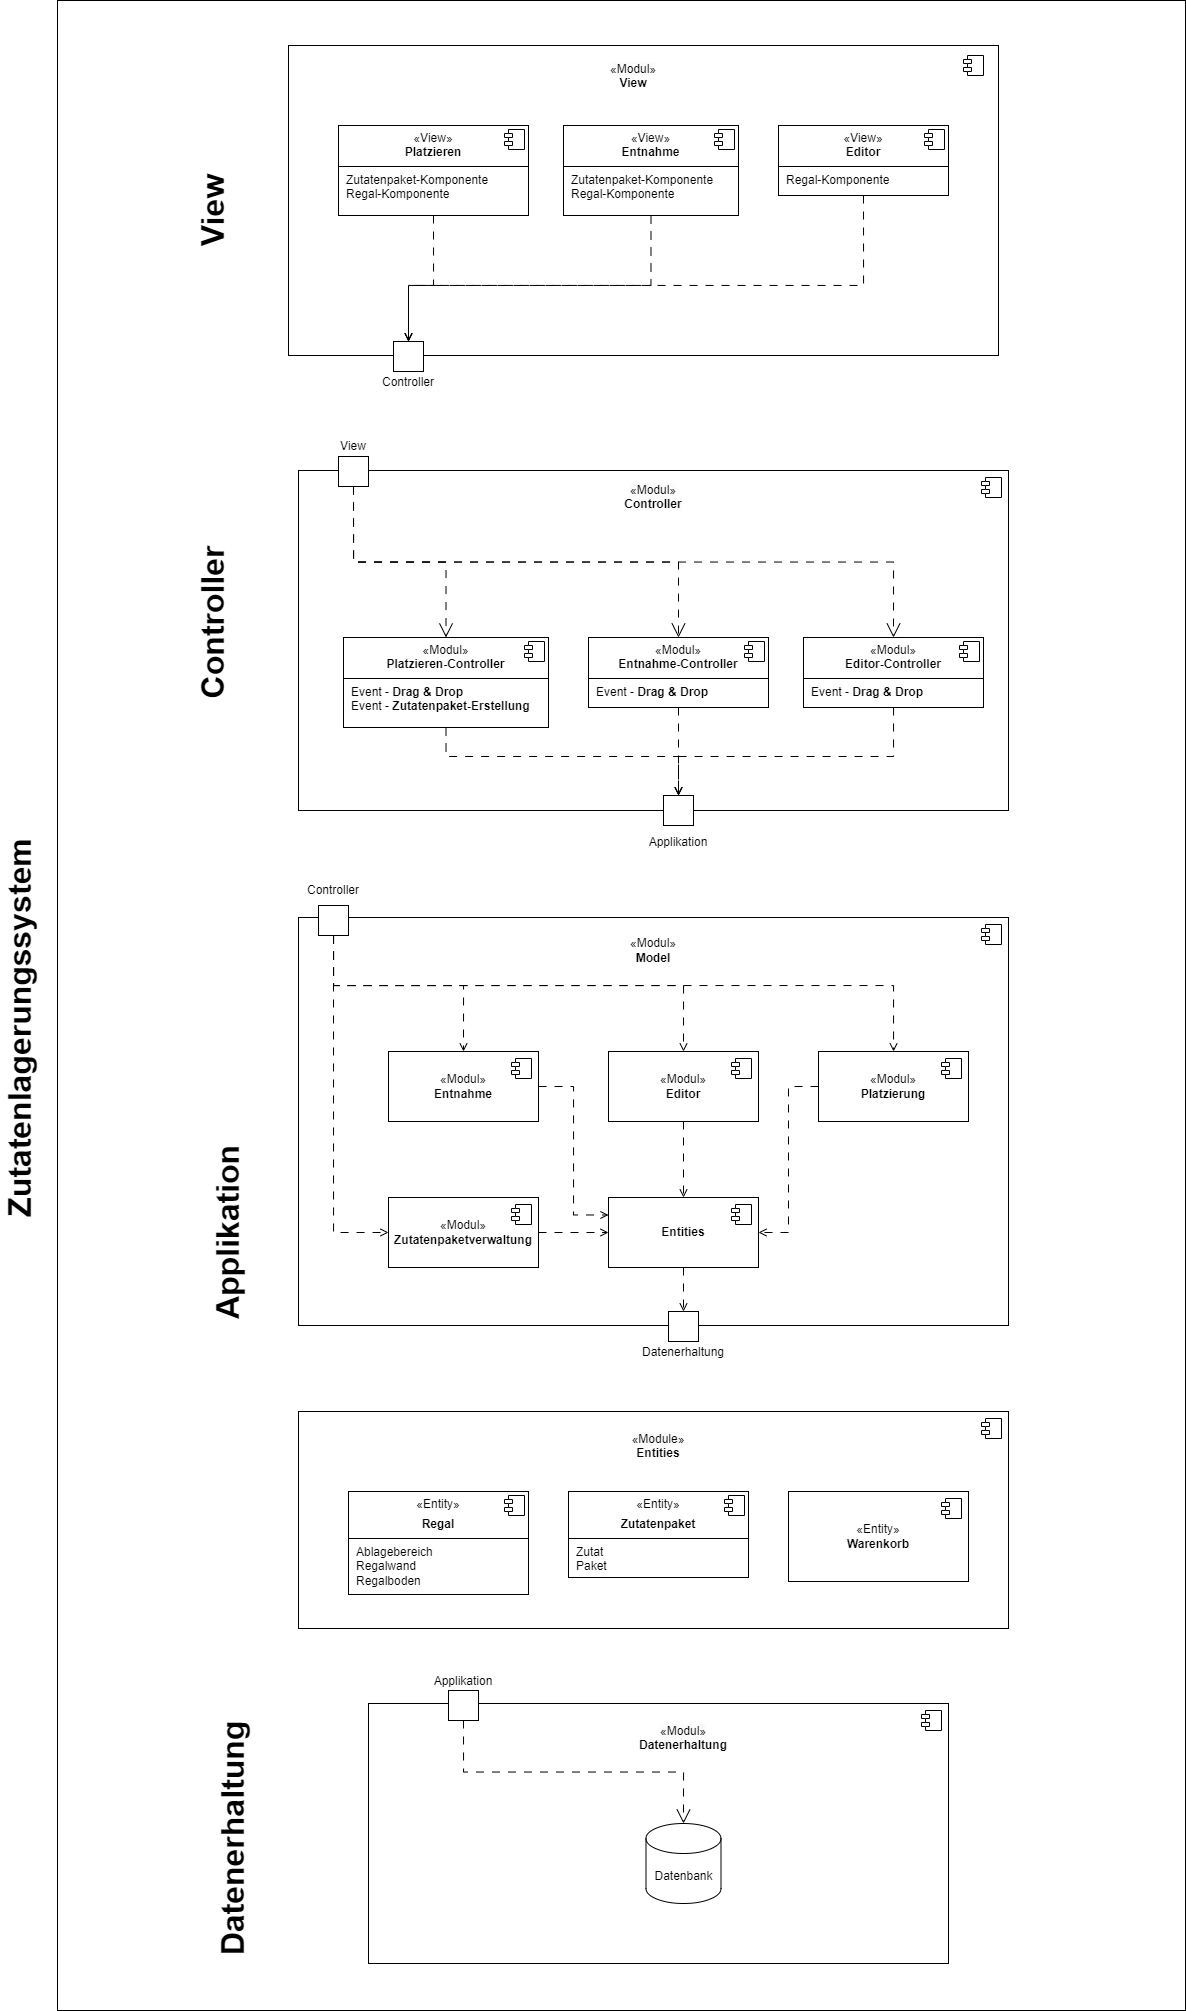
\includegraphics[width=1\textwidth]{Bilder/Kapitel/Bausteinsicht/Zutatenlagerungssystem}
    \caption{Systemübersicht}
    \label{fig:Systemuebersicht}
\end{figure}


\section{Bausteinsicht}
Dieser Abschnitt beschreibt die Zerlegung des Lagersystems in Module, wie sie sich auch in der Paketstruktur des
Java-Quellcodes widerspiegelt. Die Beschreibung konzentriert sich nur auf die Bestandteile und dessen Funktionen.
Die Module selbst verwenden Entitäten in ihren Funktionen.

\subsection{Baustein - Lager}
Die View integriert die Regal-View, welche für die Anzeige aller Regale zuständig ist. Die View wiederum ist mit dem
Editor-Controller verbunden. Der Controller hört auf Events der View. Wird ein Event durch einen User getriggert,
bekommt dies der Controller mit. Er delegiert daraufhin eventabhängig zu unterschiedlichen Methoden des
Editor-Services. Dieser kümmert sich um die Verarbeitung und Aktualisierung der Businessdaten. Veränderungen dieser
Businessdaten wiederum bekommt die View über lose Kopplung mit und aktualisiert sich daraufhin.

\begin{figure}[H]
    \centering
    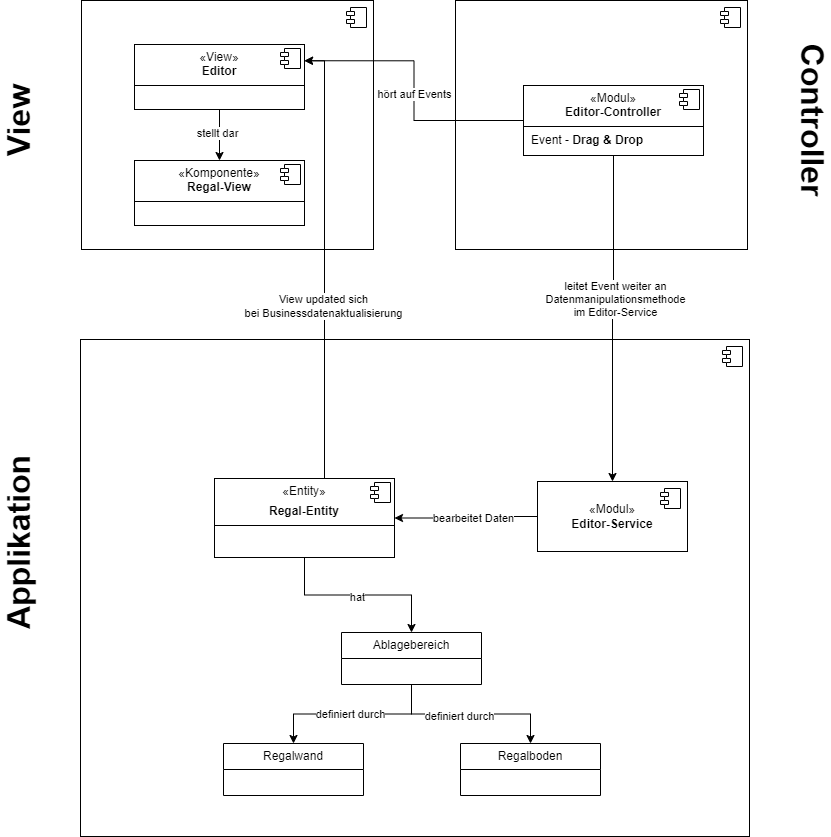
\includegraphics[width=1\textwidth]{Bilder/Kapitel/Bausteinsicht/Baustein_Editor}
    \caption{Baustein Editor}
    \label{fig:Baustein_Editor}
\end{figure}

\subsection{Baustein - Platzierung}
Für die Anzeige der Regale, der Zutatenpakete und der Such-Komponente, ist die View zuständig, welche die Platzierungs-View
integriert. Die View ist mit dem Platzierungs-Controller verbunden und dieser hört auf die Events (Drag \& Drop) der View.
Zudem bekommt er mit, wenn der User ein Event anstößt und delegiert dies eventabhängig zu den verschiedenen Methoden des
Platzierungs-Service und Zutatenpaketverwaltungs-Service. Diese kümmern sich um die Verarbeitung und Aktualisierung der
Businessdaten. Veränderungen dieser Businessdaten bekommt wiederum die View über lose Kopplung mit und aktualisiert sich daraufhin.

\begin{figure}[H]
    \centering
    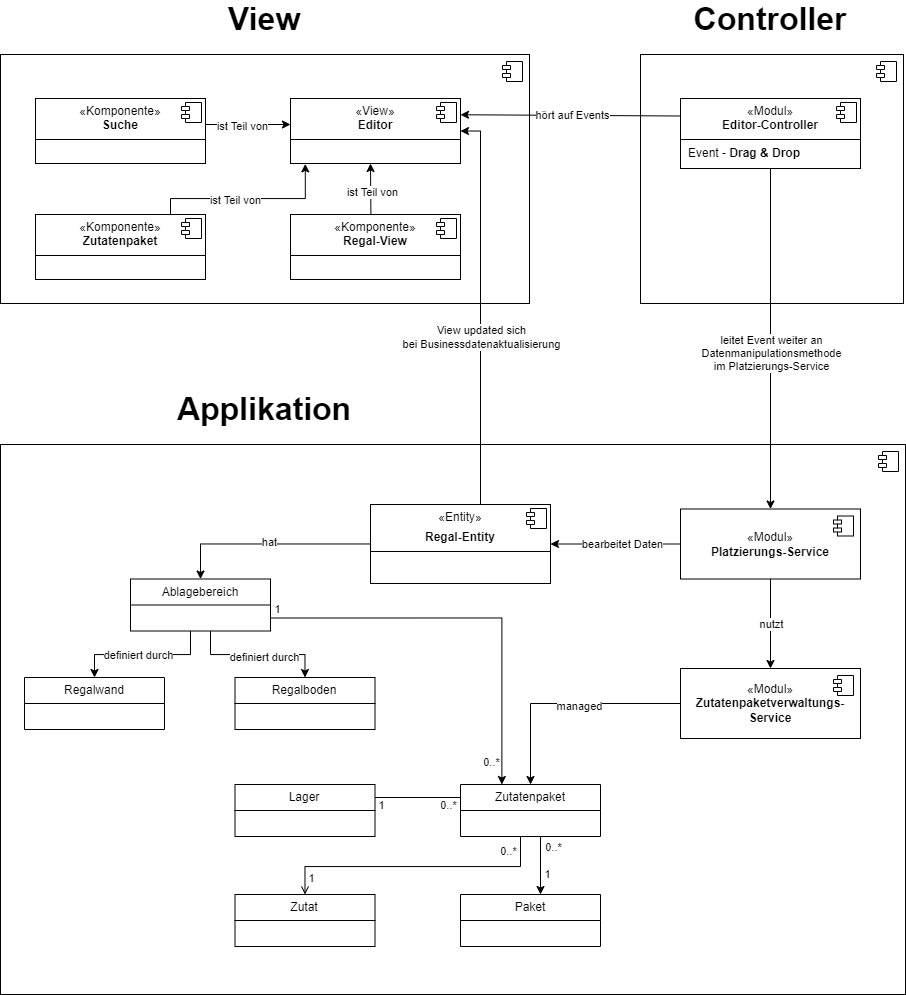
\includegraphics[width=1\textwidth]{Bilder/Kapitel/Bausteinsicht/Baustein_Platzierung}
    \caption{Baustein Platzierung}
    \label{fig:Baustein_Platzierung}
\end{figure}

\subsection{Baustein - Entnahme}
Die Entnahme-View wird in der View integriert, welche für die Anzeige aller Regale, aller Zutatenpakete und der
Such-Komponente zuständig ist. Die View ist mit dem Entnahme-Controller verbunden, der auf die Events (Drag \& Drop)
der View hört. Der Entnahme-Controller erfährt von den Events, die der User anstößt und delegiert daraufhin,
abhängig von dem angestoßenen Event, zu unterschiedlichen Methoden des Entnahme- und Zutatenpaketverwaltung-Service.
Diese kümmern sich um die Verarbeitung und Aktualisierung der Businessdaten. Der Zutatenpaketverwaltungs-Service
verwaltet den Warenkorb, der Entnahme-Service managed die Zutatenpakete. Veränderungen der Businessdaten bekommt die
View über lose Kopplung mit und aktualisiert sich daraufhin.

\begin{figure}[H]
    \centering
    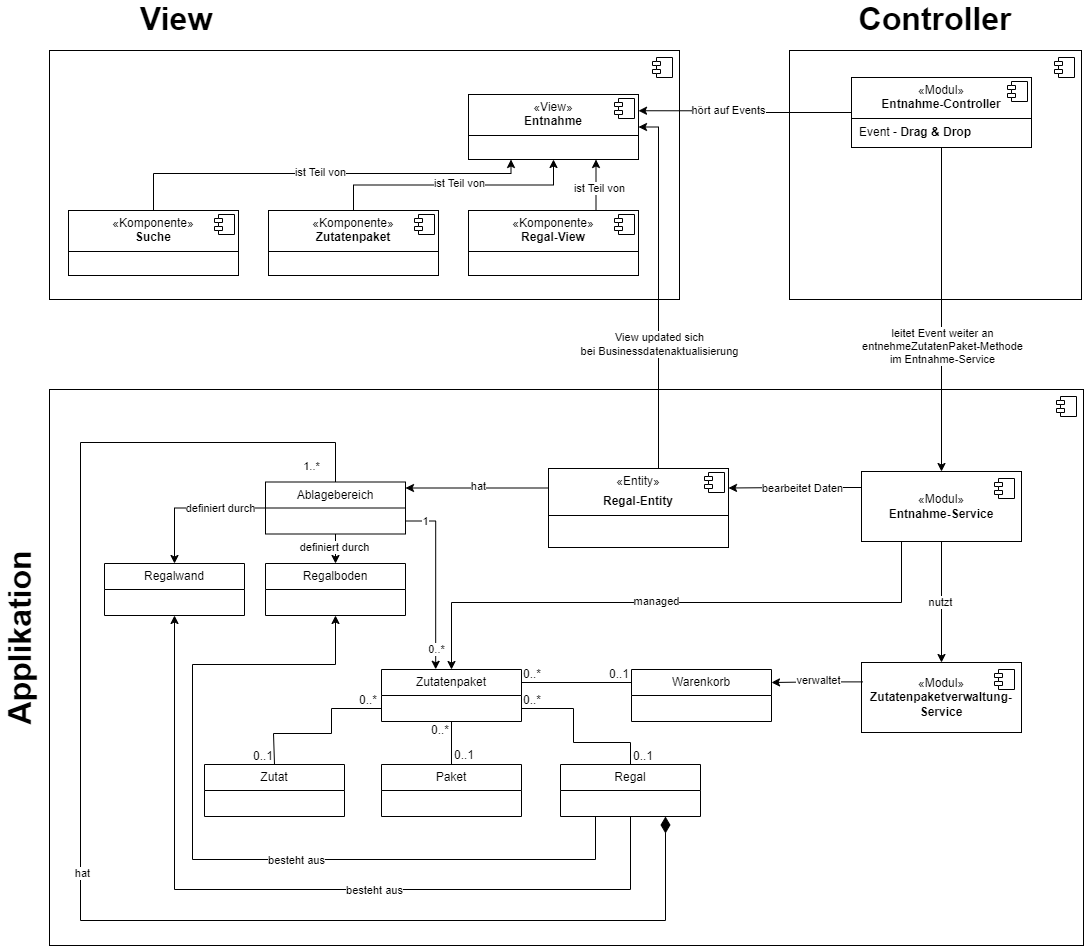
\includegraphics[width=1\textwidth]{Bilder/Kapitel/Bausteinsicht/Baustein_Entnahme}
    \caption{Baustein Entnahme}
    \label{fig:Baustein_Entnahme}
\end{figure}

\section{Servicemethoden}
\subsection{Entnahme}\label{subsec:entnahme}
\subsubsection{Zweck/Verantwortlichkeit}
Die Entnahme ist für das Entnehmen und Entfernen von Zutatenpaketen im Lager zuständig.
\subsubsection{Schnittstellen}
Die Funktionalität wird mithilfe einer Java Klasse mit dem Namen Entnahme zur Verfügung gestellt.
\begin{figure}[H]
    \centering
    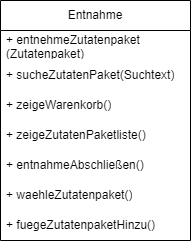
\includegraphics[width=0.3\textwidth]{Bilder/Kapitel/Bausteinsicht/Entnahme}
    \caption{Entnahme}
    \label{fig:Entnahme}
\end{figure}

\begin{table}[h]
    \centering
    \begin{tabularx}{\textwidth}{ l|X }
        \textbf{Methode} & \textbf{Kurzbeschreibung}\\
        \hline
        entnehmeZutatenPaket(ZutatenPaket) & Entfernt das Zutatenpaket aus dem Regal und fügt es dem Warenkorb hinzu\\
        \hline
        sucheZutatenpaket(Suchtext) & Möglichkeit zur Suche des gewünschten Zutatenpakets im Lager\\
        \hline
        zeigeWarenkorb() & Anzeige der bereits entnommenen Zutatenpakete\\
        \hline
        zeigeZutatenpaketliste() & Anzeige der im Lager befindlichen Zutatenpakete\\
        \hline
        entnahmeAbschließen() & Abschließen des Entnahmeprozesses und dessen Speicherung\\
        \hline
        waehleZutatenpaket() & Wählt ein Zutatenpaket aus der Zutatenpaketverwaltung aus\\
        \hline
        fuegeZutatenpaketHinzu & Fügt ein Zutatenpaket in den Warenkorb hinzu\\
    \end{tabularx}
    \caption{Entnahme Methoden}
    \label{tab:Entnahme_Methoden}
\end{table}

\subsection{Platzierung}\label{subsec:platzierung}

\subsubsection{Zweck/Verantwortlichkeit}
Das Modul Platzierung ist für die Positionsfindung der Zutatenpakete im Lager zuständig. Hierbei muss diese
beachten, dass Zutatenpakete nur dort platziert werden könne, wo Platz ist. Zutatenpakete dürfen nur auf anderen
Zutatenpakete platziert werden, wenn diese die nötige Tragfähigkeit besitzen. Außerdem dürfen Zutatenpakete nicht
mit anderen Zutatenpaketen in einem Lagerbereich mit Unverträglichkeiten zusammen sein.
\subsubsection{Schnittstellen}
Die Funktionalität wird mithilfe einer Java Klasse mit dem Namen Platzierung zur Verfügung gestellt.

\begin{figure}[H]
    \centering
    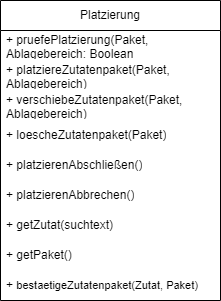
\includegraphics[width=0.3\textwidth]{Bilder/Kapitel/Bausteinsicht/Platzierung}
    \caption{Platzierung}
    \label{fig:Platzierung}
\end{figure}

\begin{table}[h]
    \centering
    \begin{tabularx}{\textwidth}{ l|X }
        \textbf{Methode} & \textbf{Kurzbeschreibung}\\
        \hline
        pruefePlatzierung(Paket, Ablagebereich): Boolean & Prüfung der Plazierung des Zutatenpakets, ob Platz
        vorhanden ist, Tragfähigkeit gegeben ist und keine Unverträgichkeiten im Lagerbereich vorhanden sind.\\
        \hline
        platziereZutatenpaket(Paket, Ablagebereich) & Entgültige Platzierung des Zutatenpakets und hinzufügen zum
        Lager\\
        \hline
        verschiebeZutatenpaket(Paket, Ablagebereich) & Verschieben des Zutatenpakets in seiner Position mit
        Bebachtung der Pruefkriterien.\\
        \hline
        loescheZutatenpaket(Paket) & Entfernen des Zutatenpakets aus dem Lager\\
        \hline
        platzierenAbschließen() & Abschließen und Speichern des Platzierprozesses\\
        \hline
        platzierenAbbrechen() & Abbrechen des Platzierprozesses und herstellen des vorherigen Zustands\\
        \hline
        getZutat(suchtext) & Holt die Zutate mit dem Titel suchtext aus der Zutatenpaketverwaltung\\
        \hline
        getPaket() & Holt das Paket aus der Zutatenpaketverwaltung\\
        \hline
        bestaetigeZutatenpaket(Zutat, Paket) & Bestätigt der Zutatenpaketverwaltung die Zutat und das Paket. Daraufhin
        wird ein neues Zutatenpaket von ihr erstellt.\\
    \end{tabularx}
    \caption{Platzierung Methoden}
    \label{tab:Platzierung_Methoden}
\end{table}

\subsection{Zutatenpaketverwaltung}\label{subsec:zutatenpaketverwaltung}

\subsubsection{Zweck/Verantwortlichkeit}
Die Zutatenpaketverwaltung dient zur Erstellung und Verwaltung von Zutaten, Paketen und Zutatenpaketen, die aus
diesen zwei Bestandteilen bestehen.
\subsubsection{Schnittstellen}
Die Funktionalität wird mithilfe einer Java Klasse mit dem Namen Zutatenpaketverwaltung zur Verfügung gestellt.

\begin{figure}[H]
    \centering
    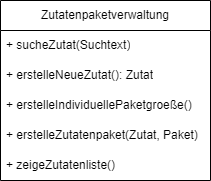
\includegraphics[width=0.3\textwidth]{Bilder/Kapitel/Bausteinsicht/Zutatenpaketverwaltung}
    \caption{Zutatenpaketverwaltung}
    \label{fig:Zutatenpaketverwaltung}
\end{figure}

\begin{table}[h]
    \centering
    \begin{tabularx}{\textwidth}{ l|X }
        \textbf{Methode} & \textbf{Kurzbeschreibung}\\
        \hline
        sucheZutat(Suchtext) & Ermöglicht die Suche nach einer vorhandenen Zutat\\
        \hline
        erstelleNeueZutat() & Erstellt eine neue Zutat und fügt sie der Zutatenliste hinzu\\
        \hline
        erstelleIndividuellePaketgroeße() & Erstellt zur den Standardmaßen von Paketen, neue individuelle Pakete.\\
        \hline
        erstelleZutatenpaket(Zutat,Paket) & Zusammen mit einem Paket und einer Zutat wird ein Zutatenpaket erstellt.\\
        \hline
        zeigeZutatenliste() & Zeigt die vorhanden Zutaten.\\
    \end{tabularx}
    \caption{Zutatenpaketverwaltung Methoden}
    \label{tab:Zutatenpaketverwaltung_Methoden}
\end{table}

\subsection{Editor}\label{subsec:editor}

\subsubsection{Zweck/Verantwortlichkeit}
Im Editor kann man das Regal im Lager mithilfe von Regalböden und Regalwänden aufbauen und diese bei Bedarf ändern.
Anhand des Aufbaus definieren sich die einzelnen Lagerbereiche. Bestehende Lager können nur editiert werden, wenn
sich keine Zutatenpakete in ihnen befinden.
\subsubsection{Schnittstellen}
Die Funktionalität wird mithilfe einer Java Klasse mit dem Namen Editor zur Verfügung gestellt.

\begin{figure}[H]
    \centering
    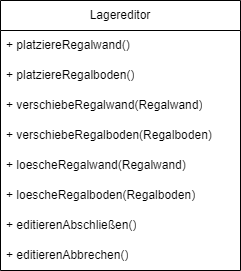
\includegraphics[width=0.3\textwidth]{Bilder/Kapitel/Bausteinsicht/Lagereditor}
    \caption{Lagereditor}
    \label{fig:Lagereditor}
\end{figure}

\begin{table}[h]
    \centering
    \begin{tabularx}{\textwidth}{ l|X }
        \textbf{Methode} & \textbf{Kurzbeschreibung}\\
        \hline
        platziereRegalwand() & Platzierung der Regalwand an geeigneten Koordinaten. Regalwände können nur vertikal
        platziert werden.\\
        \hline
        platziereRegalboden() & Platzierung des Regalbodens. Regalboden kann nur zwischen zwei Regalwänden platziert
        werden.\\
        \hline
        verschiebeRegalwand(Regalwand) & Änderung der Koordinaten der Regalwand. Anpassung der Regalböden an diese
        Änderung.\\
        \hline
        verschiebeRegalboden(Regalboden) & Änderung der Koordinaten des Regalbodens. Diese wird Vertikal zwischen
        zwei Regalwänden verschoben.\\
        \hline
        loescheRegalwand(Regalwand) & Löschen einer Regalwand. Gelöschte Regalwände löschen auch die an sich
        abstützenden Regalböden.\\
        \hline
        loescheRegalboden(Regalboden) & Löschen des Regalbodens.\\
        \hline
        editierenAbschließen & Speicherung der Änderungen des Lagers.\\
        \hline
        editierenAbbrechen & Verwerfen der Änderungen und Herstellen des ursprünglichen Zustands.\\
    \end{tabularx}
    \caption{Lagereditor Methoden}
    \label{tab:Lagereditor_Methoden}
\end{table}

\section{Laufzeitsicht}

\subsection{Sequenzdiagramm – Platzierung einer Regalwand}
Das Sequenzdiagramm im unteren Abschnitt zeigt eine exemplarische Interaktion des Systems bei der Platzierung einer Regalwand.

\begin{figure}[H]
    \centering
    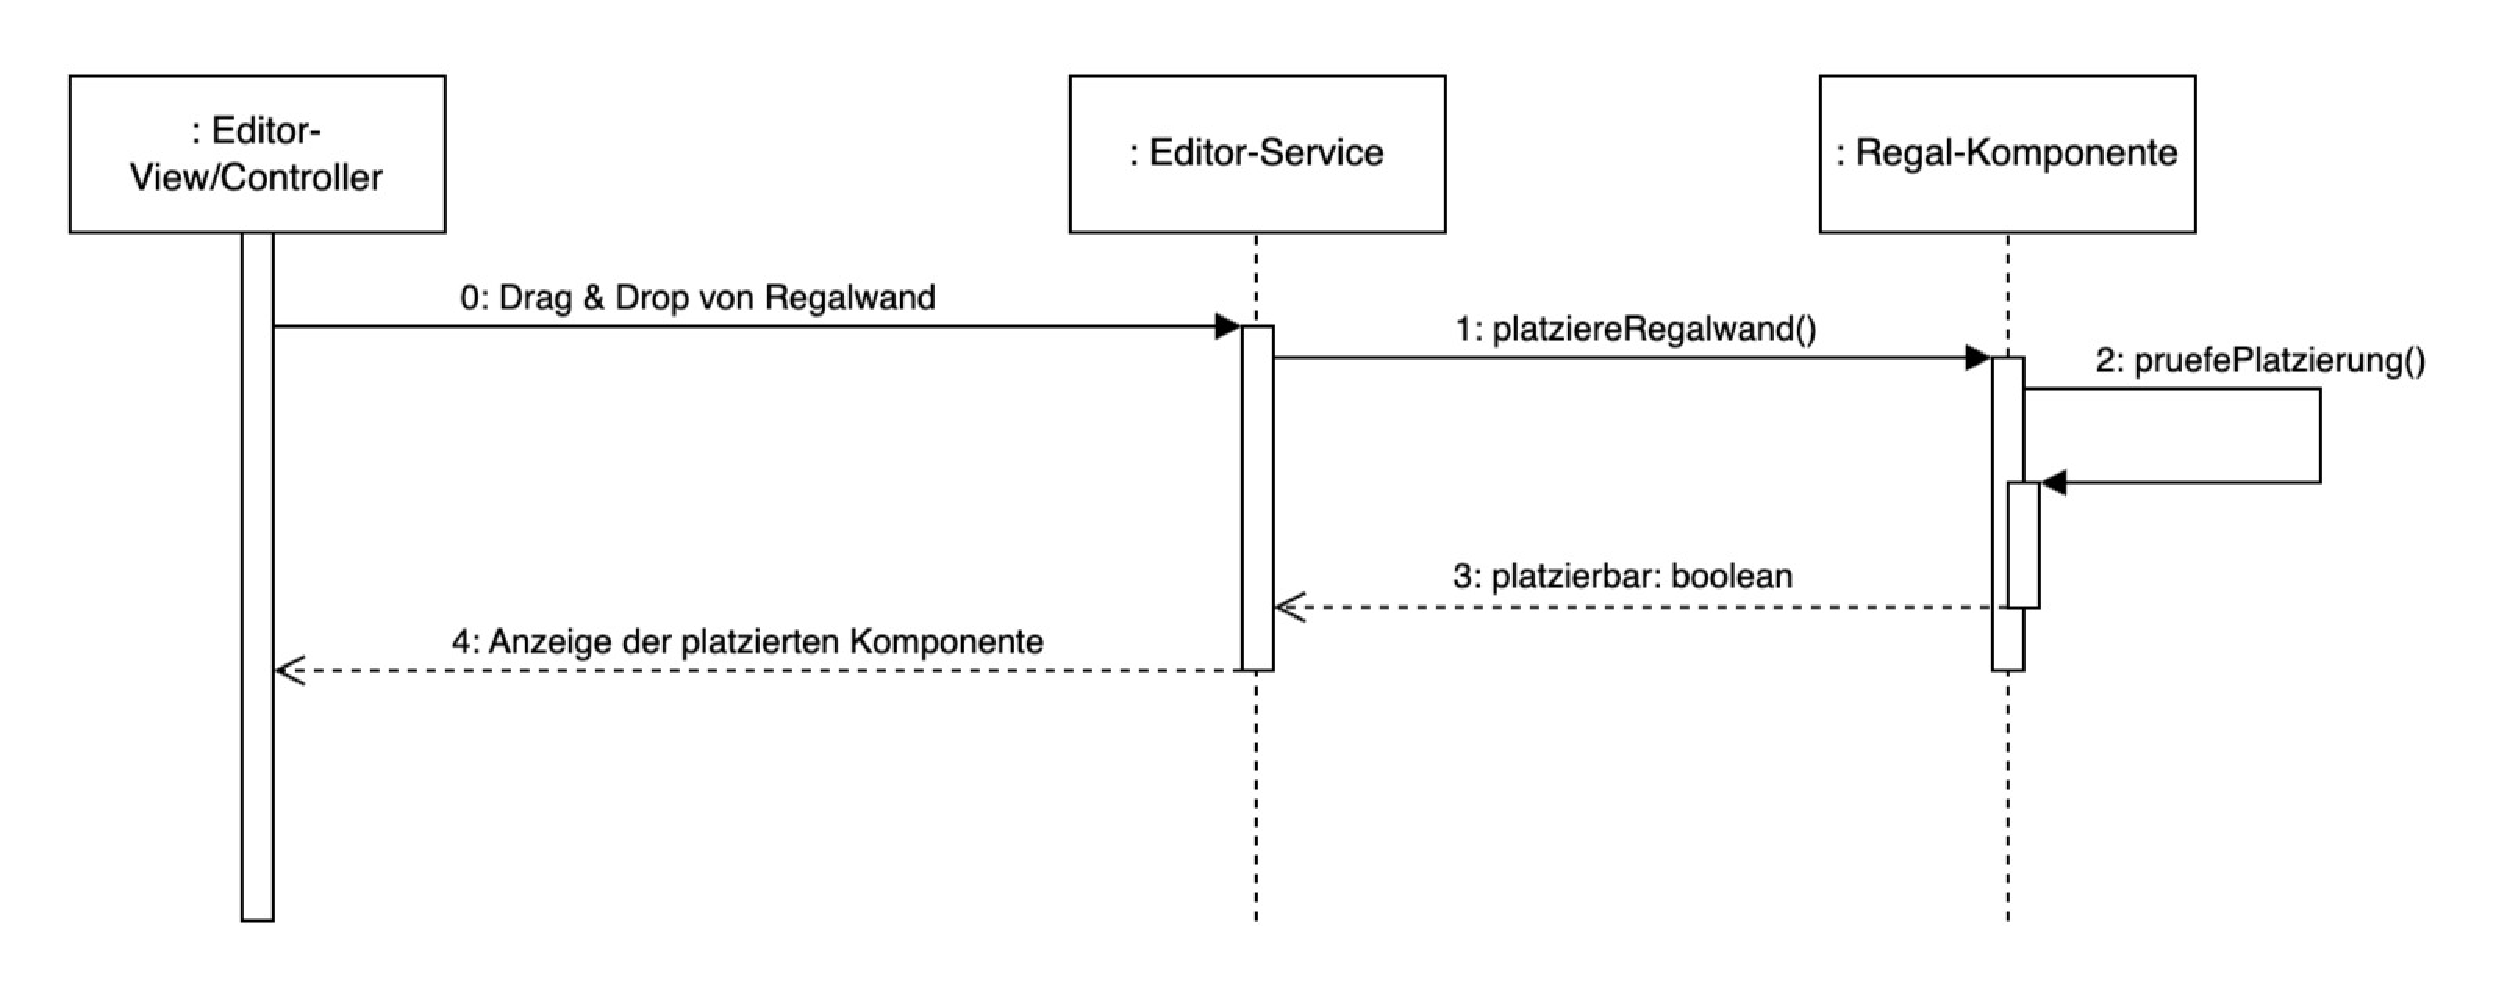
\includegraphics[width=1\textwidth]{Bilder/Kapitel/Laufzeitsicht/Sequenzdiagramm_Platzierung-Regalwand}
    \caption{Sequenzdiagramm Platzierung Regalwand}
    \label{fig:Sequenzdiagramm_Platzierung-Regalwand}
\end{figure}

Der User platziert eine Regalwand auf seine gewünschte Position in der Regalansicht, das ein Drag \& Drop-Event im
Controller auslöst. Dieses Event löst die Methode platziereRegalwand() im Editor-Service aus. Die dadurch angestoßene
Regal-Komponente prüft nun, ob die Platzierung möglich ist, mit der Methode pruefePlatzierung(). Die Regal-Komponente
gibt ein Boolean zurück. Wenn die Regalwand platzierbar ist, wird sie daraufhin platziert und in der Regalansicht
erfolgreich angezeigt.

\subsection{Sequenzdiagramm – Erstellung eines Zutatenpakets}
Das Sequenzdiagramm im folgenden Abschnitt zeigt eine exemplarische Interaktion des Systems bei der Erstellung eines Zutatenpakets.

\begin{figure}[H]
    \centering
    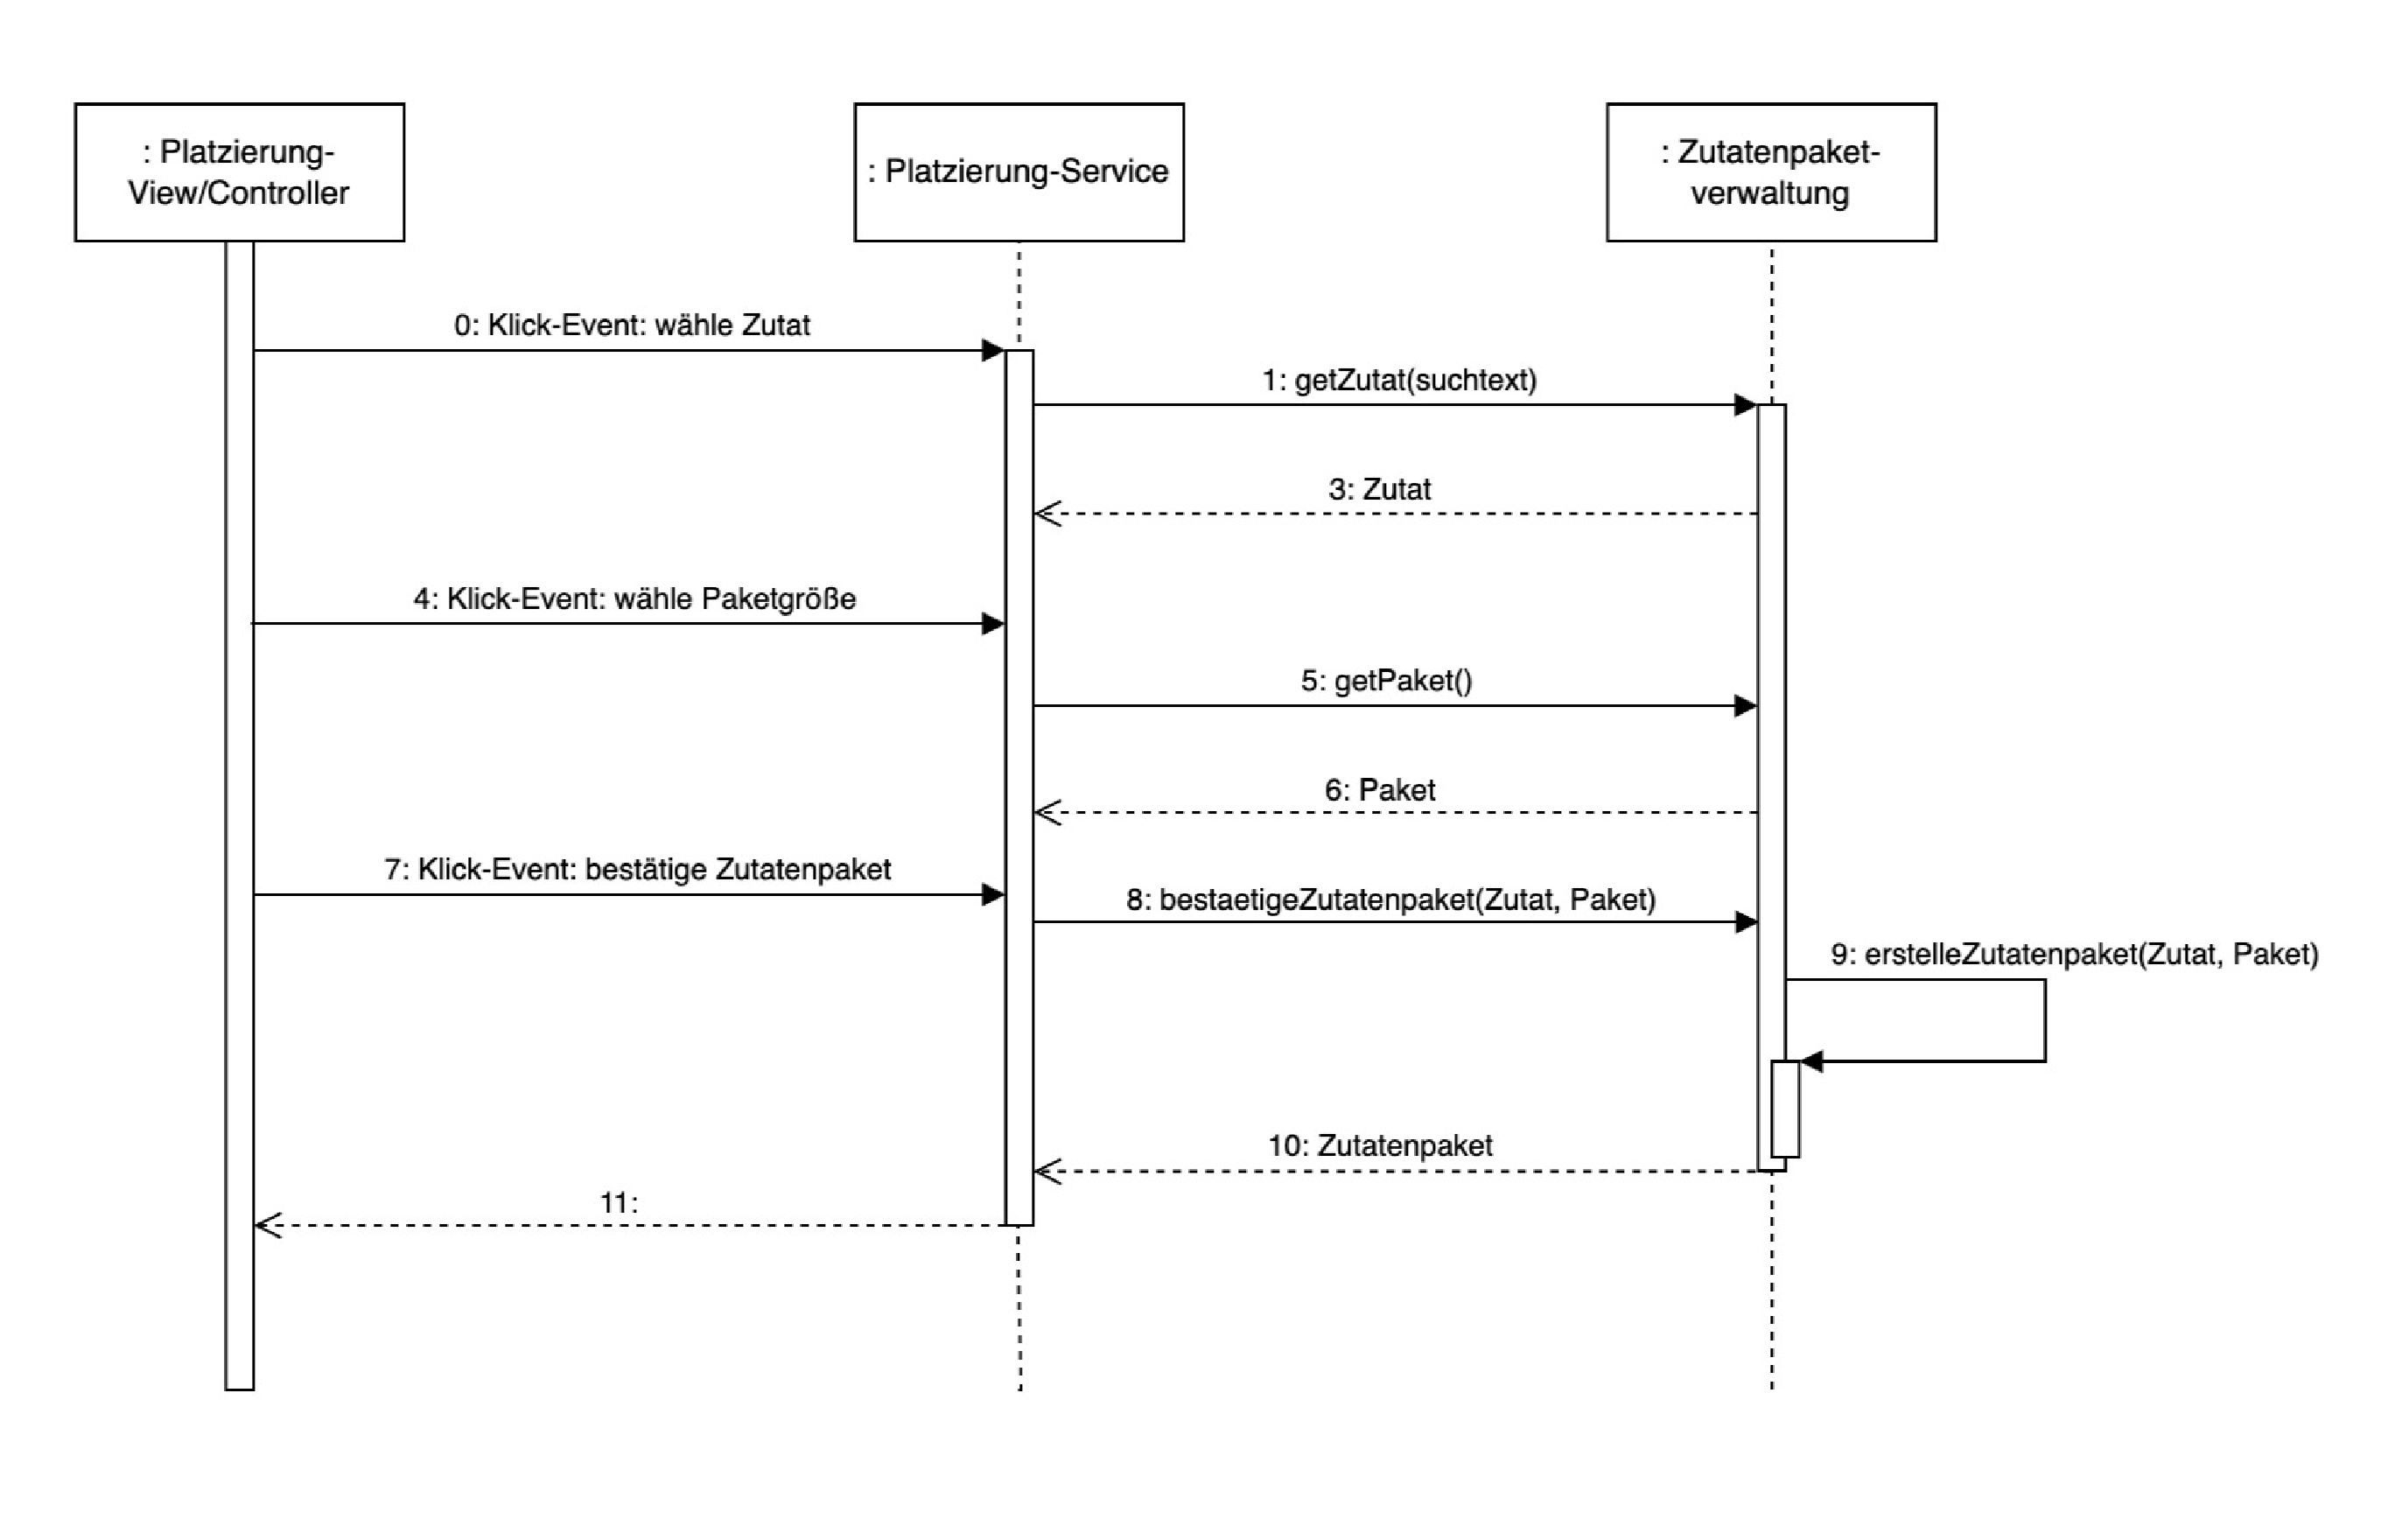
\includegraphics[width=1\textwidth]{Bilder/Kapitel/Laufzeitsicht/Sequenzdiagramm_Zutatenpaket-Erstellung}
    \caption{Sequenzdiagramm Erstellung eines Zutatenpakets}
    \label{fig:Sequenzdiagramm_Erstellung_Zutatenpaket}
\end{figure}

Durch ein Klick-Event wird eine Zutat ausgewählt. Dadurch wird in Platzierung-Service die Methode getZutat(suchtext)
ausgelöst, durch die Zutatenpaket-Verwaltung wird die gewünschte Zutat als Return zurückgegeben. Durch ein weiteres
Klick-Event wird das Paket ausgewählt, dadurch wird die Methode getPaket() im Platzierung-Service aufgerufen und die
Zutatenpaket-Verwaltung gibt das gewählte Paket als Objekt zurück. Durch das letzte Klick-Event wird das konfigurierte
Zutatenpaket bestätigt, was im Platzierung-Service die Methode bestaetigeZutatenpaket(Zutat, Paket) auslöst. In der
Zutatenpaket-Verwaltung wird das Zutatenpaket erstellt mit der Methode erstelleZutatenpaket(Zutat, Paket), welches
dann der Platzierung-Service erhällt und durch die View angezeigt wird.

\subsection{Sequenzdiagramm – Platzierung eines Zutatenpakets}
Das Sequenzdiagramm im Bild unten zeigt eine exemplarische Interaktion des Systems bei Platzierung eines Zutatenpaketes.

\begin{figure}[H]
    \centering
    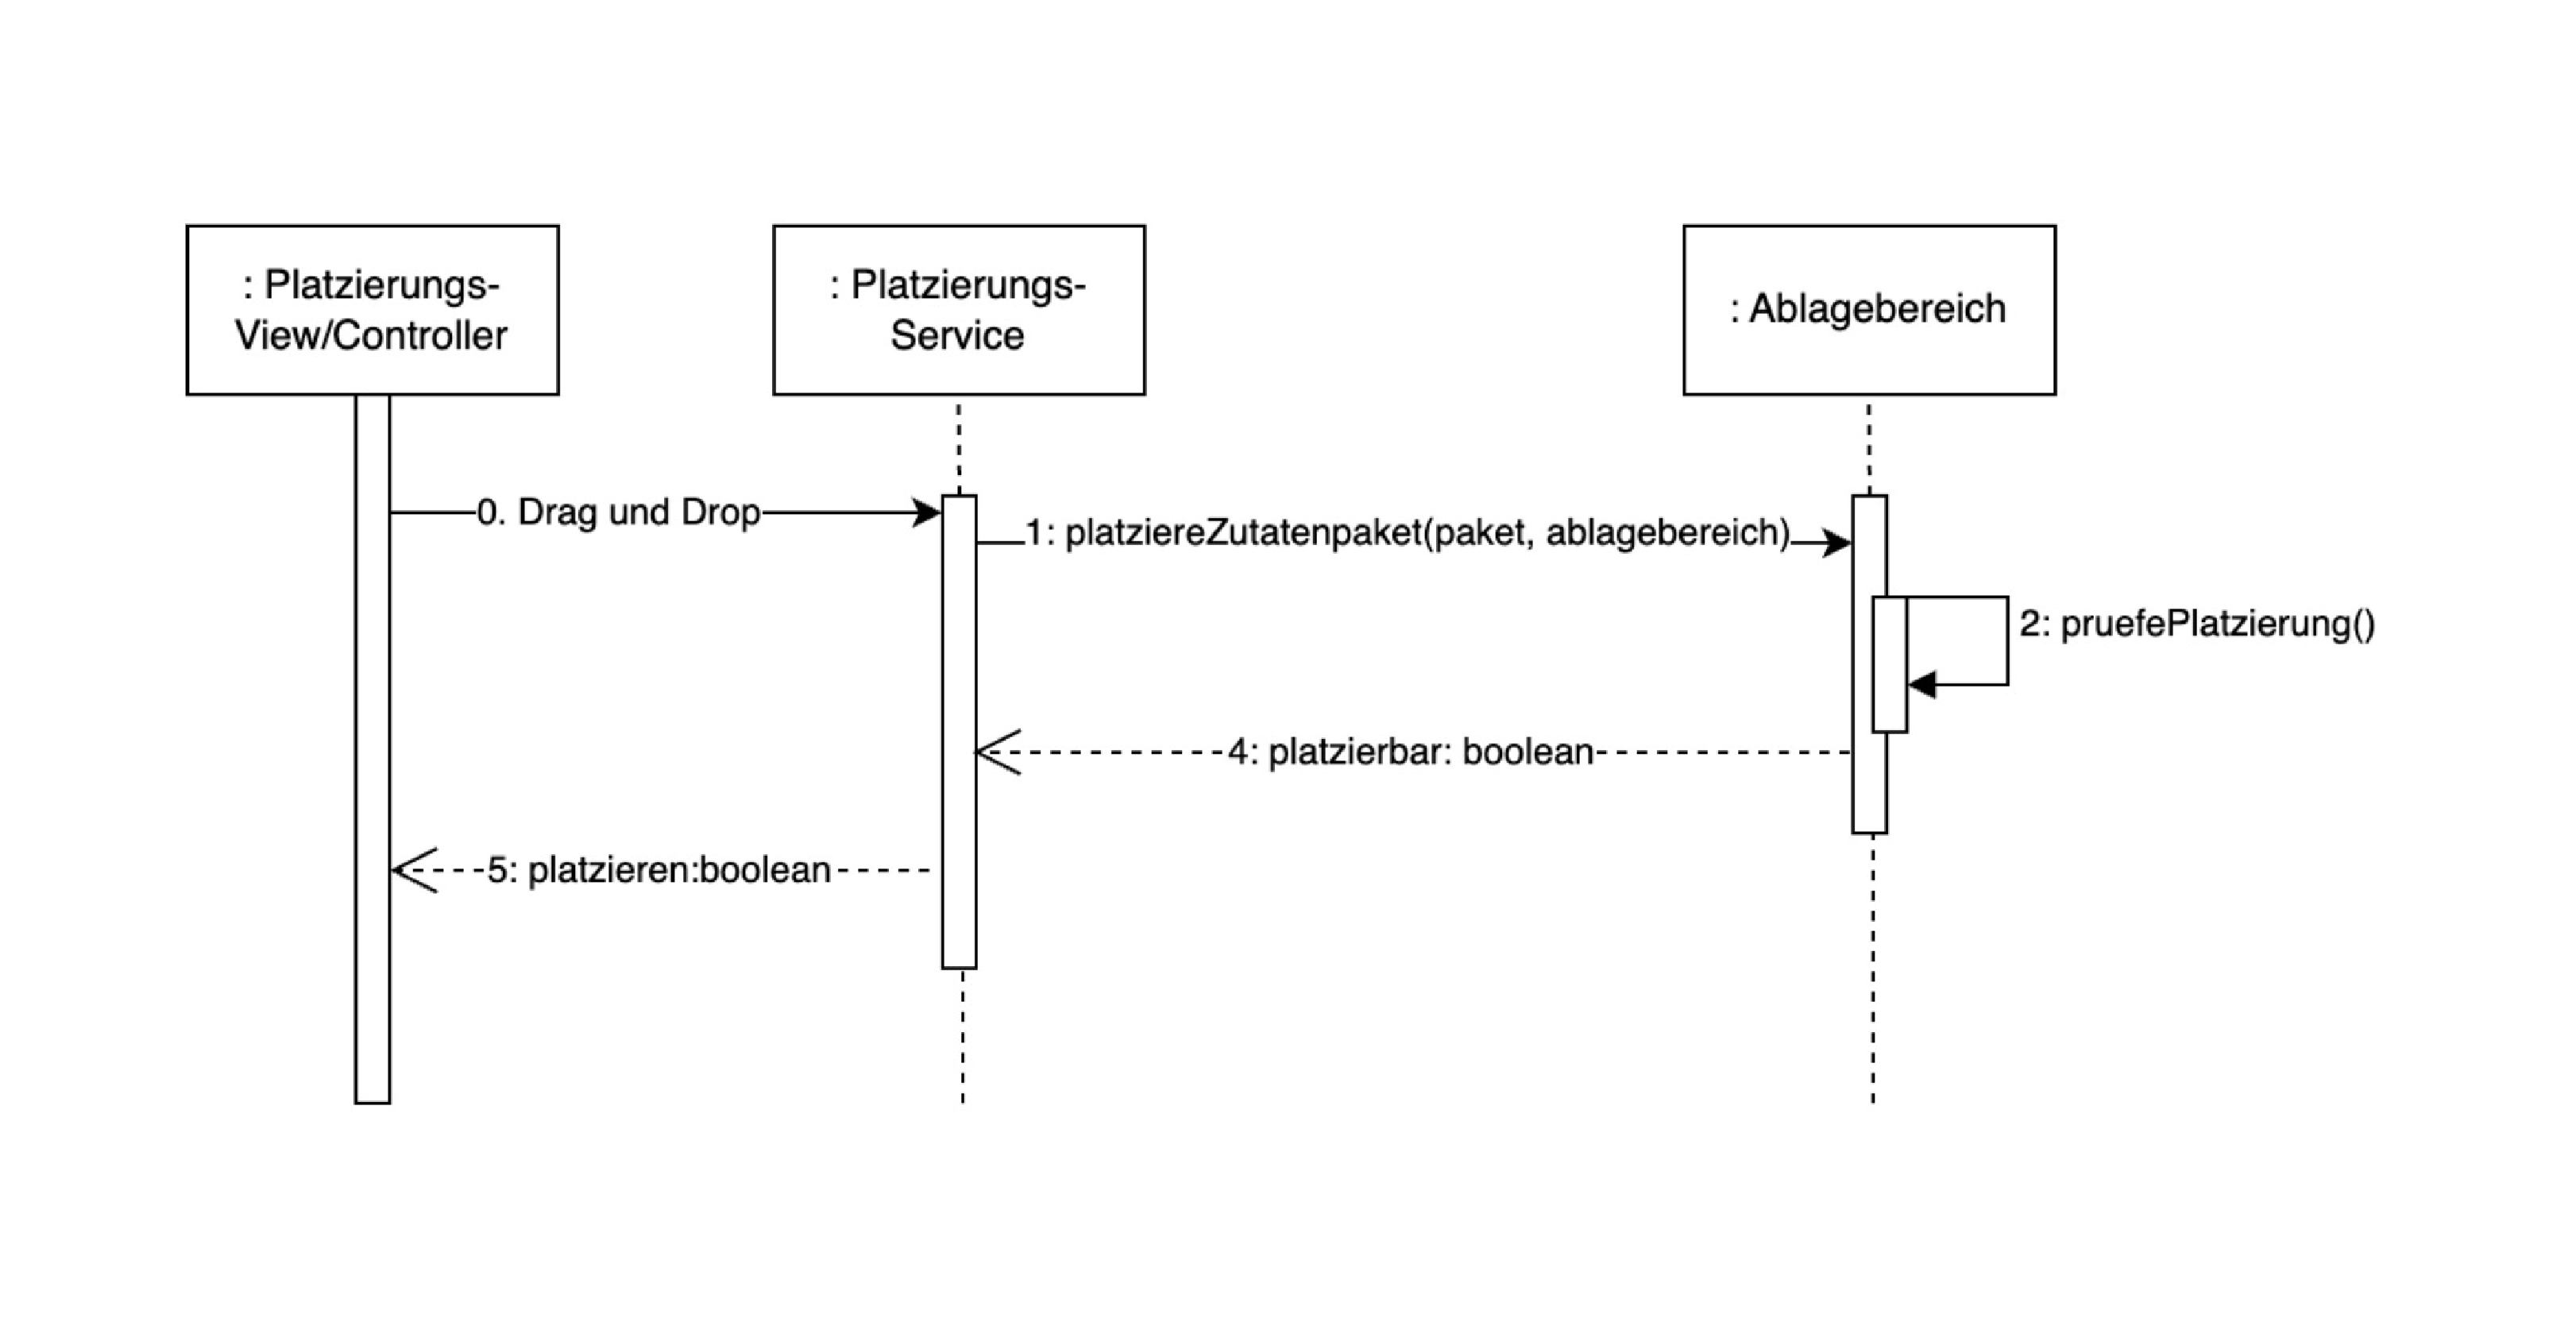
\includegraphics[width=1\textwidth]{Bilder/Kapitel/Laufzeitsicht/Sequenzdiagramm_Platzierung-Zutatenpaket}
    \caption{Sequenzdiagramm Platzierung eines Zutatenpakets}
    \label{fig:Sequenzdiagramm_Platzierung_Zutatenpaket}
\end{figure}

Zunächst zieht der User das Zutatenpaket auf einen neuen Spot, dadurch wird ein Event im Controller ausgelöst. So wird
die Methode platziereZutatenpaket(paket, ablagebereich) im Platzierung-Service ausgelöst. Diese testet nun, ob es
möglich ist, das Paket an der gewünschten Stelle zu platzieren. Dafür fragt der Ablagebereich über die Methode
pruefePlatzierung() das jeweilige Paket, welches neu platziert werden soll, ob die Größe und die Unverträglichkeiten
passen. Das Paket gibt einen Boolean zurück. Ist das Paket laut diesem platzierbar, wird im letzten Schritt das Paket
platziert. Ist das Paket nicht platzierbar, wird dies im Ablagebereich angezeigt.

\subsection{Sequenzdiagramm – Entnahme eines Zutatenpakets}
Das Sequenzdiagramm im darunter liegenden Abschnitt zeigt eine exemplarische Interaktion des Systems bei der Entnahme eines Zutatenpakets.

\begin{figure}[H]
    \centering
    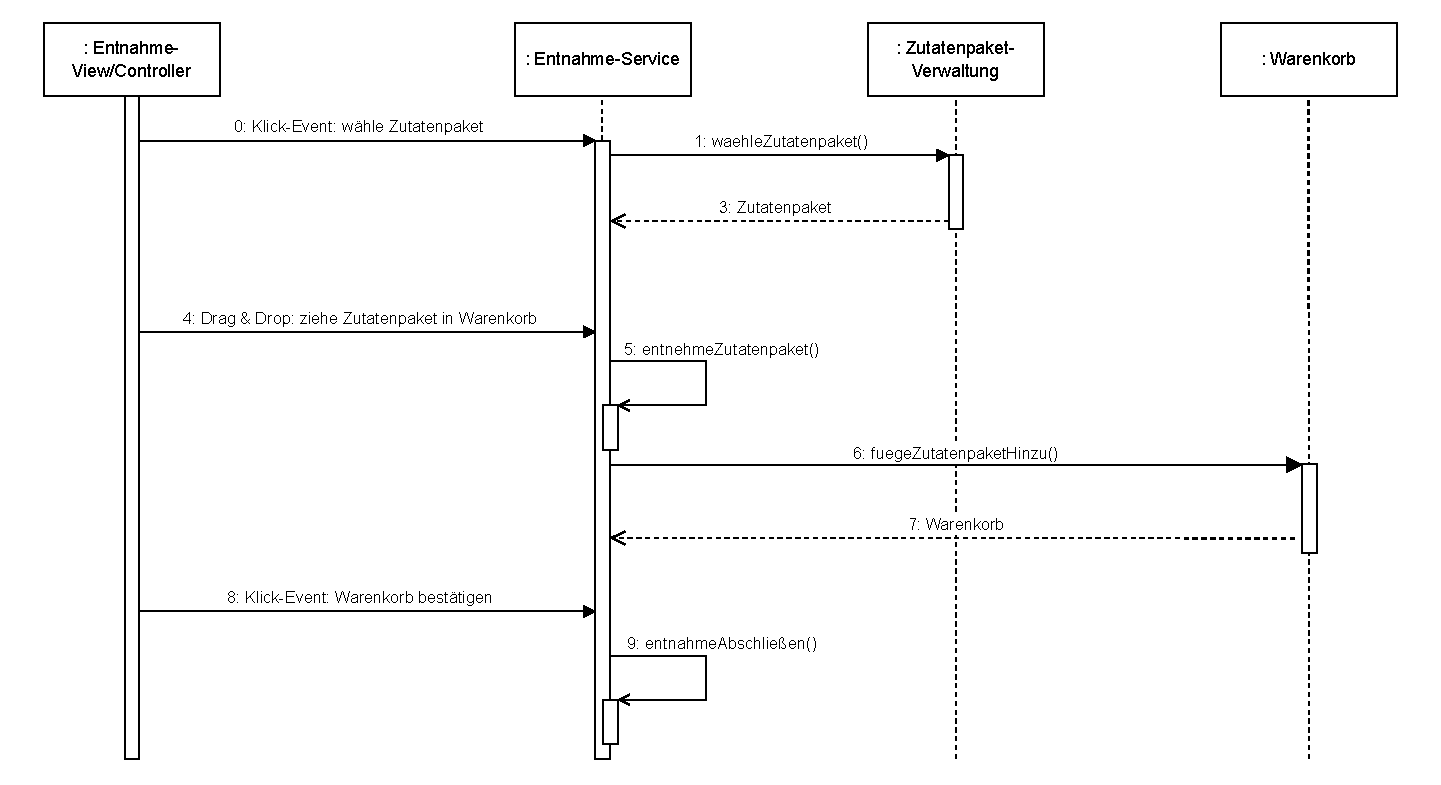
\includegraphics[width=1\textwidth]{Bilder/Kapitel/Laufzeitsicht/Sequenzdiagramm_Entnahme-Zutatenpaket}
    \caption{Sequenzdiagramm Entnahme eines Zutatenpakets}
    \label{fig:Sequenzdiagramm_Entnahme_Zutatenpaket}
\end{figure}

Als erstes wählt der User, durch ein Klick-Event, das gewünschte Zutatenpaket aus, welches er entnehmen möchte. Daraufhin
wird die Methode waehleZutatenpaket() vom Entnahme-Service angestoßen. Die Zutatenpaket-Verwaltung gibt anschließend
ein Zutatenpaket als Return zurück. Per Drag \& Drop kann der User dann das Zutatenpaket in den Warenkorb ziehen.
Dadurch prüft der der Entnahme-Service, ob die Entnahme möglich ist mit der Methode entnehmeZutatenpaket(). Im Anschluss stößt
der Entnahme-Service die Methode fuegeZutatenpaketHinzu() an, worauf der Warenkorb einen Warenkorb als Return liefert.
Durch ein weiteres Klick-Event bestätigt der User den Warenkorb. Der Entnahme-Service schließt zum Schluss mit der Methode
entnahmeAbschließen() das Event ab.

% Ende der Datei
